
%----------------------------------------------------------------------------------------
%	PACKAGES AND DOCUMENT CONFIGURATIONS
%----------------------------------------------------------------------------------------

\documentclass[https://www.overleaf.com/project/63761df255a8a9f4a15c3579
	letterpaper, % Paper size, specify a4paper (A4) or letterpaper (US letter)
	10pt, % Default font size, specify 10pt, 11pt or 12pt
]{CSUniSchoolLabReport}

\usepackage{fontawesome}
\usepackage{hyperref}
\usepackage[normalem]{ulem}
\usepackage{listings}
\usepackage{xcolor}
\definecolor{codegreen}{rgb}{0,0.6,0}
\definecolor{codegray}{rgb}{0.5,0.5,0.5}
\definecolor{codepurple}{rgb}{0.58,0,0.82}
\definecolor{backcolour}{rgb}{1,1,1}
\lstdefinestyle{mystyle}{
    backgroundcolor=\color{backcolour},   
    commentstyle=\color{codegreen},
    keywordstyle=\color{magenta},
    numberstyle=\tiny\color{codegray},
    stringstyle=\color{codepurple},
    basicstyle=\ttfamily\footnotesize,
    breakatwhitespace=false,         
    breaklines=true,                 
    captionpos=b,                    
    keepspaces=true,                 
    numbers=left,                    
    numbersep=5pt,                  
    showspaces=false,                
    showstringspaces=false,
    showtabs=false,                  
    tabsize=2
}

\lstset{style=mystyle}
\renewcommand\ULthickness{1.0pt}   %%---> For changing thickness of underline
\setlength\ULdepth{1.3ex}%\maxdimen ---> For changing depth of underline

%----------------------------------------------------------------------------------------
%	REPORT INFORMATION
%----------------------------------------------------------------------------------------


\begin{document}

\begin{figure}[H] % [H] forces the figure to be placed exactly where it appears in the text
	\centering % Horizontally center the figure
	
\includegraphics[width=0.4\textwidth]{images/logo.png} % Include the figure
\end{figure}

\begin{center}
    \begin{tabular} {c}
        \Huge Universidad La Salle \\\\\\\\
        \huge Compiladores \\\\\\\\
        \LARGE Informe de la Práctica 04 \\\\\\\\
        \huge Autómatas y Expresiones Regulares \\\\\\\\
        \LARGE Karlo Emigdio Pacha Curimayhua \\\\\\\\
        \LARGE Sexto Semestre - Ingeniería de Software \\\\\\\\
        \LARGE 2023
      \end{tabular}
\end{center}

\begin{center}
	\begin{tabular}{l r}
	\end{tabular}
\end{center}

%----------------------------------------------------------------------------------------
%	Ejercicio 1
%----------------------------------------------------------------------------------------

\section*{Ejercicio 1 }

\subsection*{Enunciado}
Convierta el siguiente AFND a un AFD. Detalle todo el desarrollo, puede incluir fotos si lo hizo en papel. (7 puntos)

\begin{figure}[H]
	\centering
	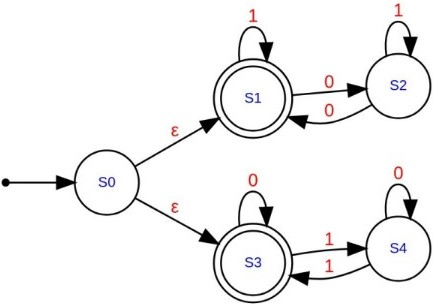
\includegraphics[width=0.5\textwidth]{images/one.jpg}
\end{figure}

%%%%%%%%%%%%%%%%%%%%%%%%%%%%%%%%%%%%%%%%
\subsection*{Solución}

\subsubsection*{Tabla de transiciones AFND}
\begin{tabular}{|c|c|c|c|}
\hline
States & 0 & 1 & \epsilon \\
\hline
>S0 & \emptyset & \emptyset &  \{S1,S3\} \\
\hline
*S1 & S2 & S1 & S1 \\
\hline
S2 & S1 & S2 & \emptyset \\
\hline
*S3 & S3 & S4 & S3 \\
\hline
S4 & S4 & S3 & \emptyset \\
\hline
\end{tabular}

%%%%%%%%%%%%%%%%%%%%%%%%%%%%%%%%%%%%%%%%
\subsubsection*{Tabla de transiciones AFD}
\begin{tabular}{|c|c|c|}
\hline
States & 0 & 1 \\
\hline
>*\{S0,S1,S3\} & \{S2,S3\} &  \{S1,S4\} \\
\hline
*\{S2,S3\} & \{S1,S3\} & \{S2,S4\} \\
\hline
*\{S1,S4\} & \{S2,S4\} & \{S1,S3\} \\
\hline
*\{S1,S3\} & \{S2,S3\} & \{S1,S4\} \\
\hline
\{S2,S4\} & \{S1,S4\} & \{S2,S3\} \\
\hline
\end{tabular}

%%%%%%%%%%%%%%%%%%%%%%%%%%%%%%%%%%%%%%%%
\subsubsection*{Tabla de transiciones AFD (Renombrando Estados)}
Para tener mejor control y lectura del AFD, es recomendable renombrar los estados.\\

\begin{tabular}{|c|c|c|}
\hline
States &  \\
\hline
>*\{S0,S1,S3\} & A \\
\hline
*\{S2,S3\} & B \\
\hline
*\{S1,S4\} & C \\
\hline
*\{S1,S3\} & D \\
\hline
\{S2,S4\} & E \\
\hline
\end{tabular}

%%%%%%%%%%%%%%%%%%%%%%%%%%%%%%%%%%%%%%%%
\subsubsection*{AFD inicial}

\begin{tabular}{|c|c|c|}
\hline
>*A & B & C \\
\hline
*B & D & E \\
\hline
*C & E & D \\
\hline
*D & B & C \\
\hline
E & C & B \\
\hline
\end{tabular}

\begin{figure}[H]
	\centering
	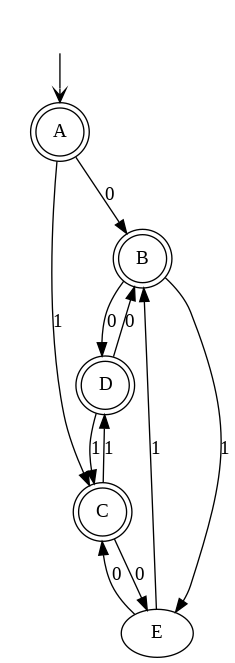
\includegraphics[width=0.35\textwidth]{images/automata1.png}
    \caption{AFD inicial}
\end{figure}


%%%%%%%%%%%%%%%%%%%%%%%%%%%%%%%%%%%%%%%%
\subsubsection*{AFD final (reducido)}
Si bien el autómata parece estar terminado, se le puede aplicar una reducción. El estado D tiene transiciones a B y C que no son necesarias ya que ambos estados son estados finales o de aceptación, basta con redireccionar esas transiciones hacia A.\\

\begin{tabular}{|c|c|c|}
\hline

States & 0 & 1 \\
\hline
>*A & B & C \\
\hline
*B & A & D \\
\hline
*C & D & A \\
\hline
D & C & B \\
\hline
\end{tabular}

\begin{figure}[H]
	\centering
	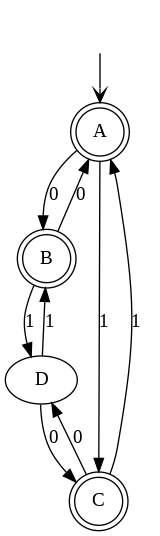
\includegraphics[width=0.27\textwidth]{images/automata2.png}
    \caption{AFD final}
\end{figure}

%%%%%%%%%%%%%%%%%%%%%%%%%%%%%%%%%%%%%%%%


%%%%%%%%%%%%%%%%%%%%%%%%%%%%%%%%%%%%%%%%
\subsection*{Código para graficar los Autómatas}
\lstinputlisting[language=python]{codes/grapher.py}

\\\\
%------------------------------------------------------------------------------------------------------------
%	Ejercicio 2
%------------------------------------------------------------------------------------------------------------

\section*{Ejercicio 2 }

\subsection*{Enunciado}
Normalmente para reconocer una expresión regular se siguen los siguientes pasos:\\

\begin{itemize}
  \item Convertir la expresión regular a un Automata Finito No Determinista (AFND).
  \item El AFND debe ser transformado a un Automata Finito Determinista (AFD).
  \item Finalmente este AFD, es representado mediante una tabla de transiciones.
  \item Se implementa un programa para reconocer las ocurrencias de una expresi ́on regular utilizando la tabla de transiciones.
\end{itemize}
\\\\
En esta caso, le brindamos el AFD para reconocer identificadores, se le pide obtener la tabla de transiciones e implementar un programa en Python que tome esta tabla (la puedes definir estáticamente) y reconozca los identificadores de un archivo de texto (similar a la función findall de python). (11 puntos)

\begin{figure}[H]
	\centering
	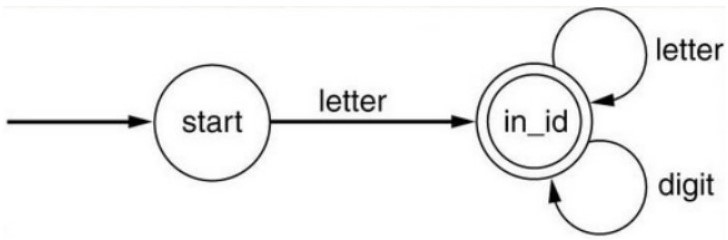
\includegraphics[width=0.5\textwidth]{images/two.jpg}
\end{figure}

%%%%%%%%%%%%%%%%%%%%%%%%%%%%%%%%%%%%%%%%
\subsection*{Solución 1}
Esta solución no usa Regex en las transiciones, pero cumple satisfactoriamente con lo esperado.

%%%%%%%%%%%%%%%%%%%%%%%%%%%%%%%%%%%%%%%%
\subsubsection*{Código para Strings)}
\lstinputlisting[language=python]{codes/main2.py}
\begin{figure}[H]
	\centering
	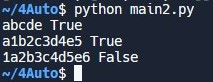
\includegraphics[width=0.65\textwidth]{images/1.jpg}
\end{figure}
%%%%%%%%%%%%%%%%%%%%%%%%%%%%%%%%%%%%%%%%
\\\\
\subsubsection*{Código para lectura de archivos(ds) y salida txt }
\lstinputlisting[language=python]{codes/main4.py}

%%%%%%%%%%%%%%%%%%%%%%%%%%%%%%%%%%%%%%%%

\subsection*{Solución 2}
Esta solución usa Regex en las transiciones y cumple satisfactoriamente con lo esperado, aunque al seguir la lógica del código proporcionado, tiene mayor gasto de recursos y tiempo.

%%%%%%%%%%%%%%%%%%%%%%%%%%%%%%%%%%%%%%%%
\subsubsection*{Código para Strings}
\lstinputlisting[language=python]{codes/main3.py}

\begin{figure}[H]
	\centering
	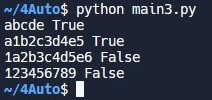
\includegraphics[width=0.5\textwidth]{images/2.jpg}
\end{figure}
%%%%%%%%%%%%%%%%%%%%%%%%%%%%%%%%%%%%%%%%
\\\\
\subsubsection*{Código para lectura de archivos(ds) y salida txt }
\lstinputlisting[language=python]{codes/main.py}

%%%%%%%%%%%%%%%%%%%%%%%%%%%%%%%%%%%%%%%%
\subsection*{Entrada y Salida de archivos para las soluciones completas}
%%%%%%%%%%%%%%%%%%%%%%%%%%%%%%%%%%%%%%%%
\subsubsection*{Entrada 1}
\lstinputlisting[language=javascript]{codes/example.ds}
\subsubsection*{Salida 1}
\lstinputlisting[language=txt]{codes/out1.txt}
%%%%%%%%%%%%%%%%%%%%%%%%%%%%%%%%%%%%%%%%
\subsubsection*{Entrada 2}
\lstinputlisting[language=javascript]{codes/example2.ds}
\subsubsection*{Salida 2}
\lstinputlisting[language=txt]{codes/out2.txt}
%----------------------------------------------------------------------------------------
\\
\\
\\
\href{https://github.com/DAOBLUR/CompilersPractices/tree/main/4}{\huge\faGithub \textbf{{Repositorio GitHub}} }


\end{document}